\section{Initial and boundary conditions}\label{pocatecni a okrajove podminky}

The appropriate choice of initial and boundary conditions, consistent with the studied problem, is an integral part of the subsequent numerical simulation. Due to the specific mesoscopic description of the fluid within LBM, careful attention must be given to the initial and boundary conditions used in the practical part of this work. Therefore, the chosen initial and boundary conditions are described in more detail below.

\subsection{Initial condition}\label{pocatecni podminka}
Let us now consider the domain defined by relations \eqref{eq:domain}. To set the initial condition, we use the equilibrium distribution function \( f^{\mathrm{eq}} \), which has the form
\begin{equation}\label{eq:feq}
	f^{\mathrm{eq}}_{k} = \rho w_{k} \, \left(1 + \frac{\vec{\xi_{k}} \cdot \vec{u}}{c^{2}_{s}} + \frac{(\vec{\xi_{k}} \cdot \vec{u})^2}{2c^{4}_{s}} - \frac{\vec{u} \cdot \vec{u}}{2c^{2}_{s}} \right)\, , \hspace{2mm} k \in \{1,\dots,27\},
\end{equation}
where \( w_{k} \) represents the weights specific to the chosen velocity model. For the D3Q27 model, these weights are given as \cite{Kruger}
\begin{equation}
	w_k= \begin{cases}\frac{8}{27}, & k=1, \\ \frac{2}{27}, & k = 2,3, \ldots, 7, \\ \frac{1}{54}, & k = 8,9, \ldots, 19, \\ \frac{1}{216}, & k = 20,21, \ldots, 27.\end{cases}
\end{equation}
The initial distribution \( \rho \), and the velocity \( \vec{u} \), are defined as \( \rho _{\mathrm{ini}} \) and \( \vec{u} _{\mathrm{ini}} \), respectively. Then, for each node \( \vec{x} \in \hat{\Omega} \) at time \( t=0 \), we have

\begin{equation}\label{eq:initial condition}
	f^{}_{k} (\vec{x}, 0) = f^{\mathrm{eq}}_{k} (\rho _{\mathrm{ini}} (\vec{x}), \vec{u} _{\mathrm{ini}} (\vec{x})), \hspace{3mm} k \in \{1, \dots 27\}.
\end{equation}
In this approach to setting the initial condition, we assume that the non-equilibrium part of the distribution functions \( f^{\mathrm{neq}}_{k} = f_{k} - f^{\mathrm{eq}}_{k} \) can be neglected, and the distribution functions can be approximated by their equilibrium part. A significant advantage of this choice of initial condition approximation is its straightforward implementation, and therefore, it is used in this work, although other more sophisticated options exist, such as those discussed in \cite{PE}.

\subsection{Boundary conditions}


\subsubsection{Bounce-back boundary condition}\label{bounce-back}
The first boundary condition discussed is the bounce-back boundary condition, specifically its \textit{fullway} variant. The bounce-back boundary condition is typically used at the interface between a fluid and a solid. Its advantage is that it satisfies the no-slip boundary condition at the interface, and its implementation is straightforward. The principle of the bounce-back boundary condition is that at the interface, the distribution functions corresponding to particles with microscopic velocity \( \vec{\xi_{k}} \) are reflected back into the directions from which they arrived at the node, with velocity \( \vec{\xi_{\bar{k}}} = -\vec{\xi_{k}} \).

When using this boundary condition, the interface is located halfway between the fluid and solid nodes. This does not cause issues when modeling flow around straight walls parallel to the grid, but for curved boundaries that are not parallel to the grid, the bounce-back method leads to a "staircase" shape of the boundary, which does not provide a good approximation of the actual interface position.

The fullway variant of the bounce-back boundary condition requires two time steps for the reflection of the hypothetical particles. During this time, the particles travel to the solid nodes, where their direction is reversed in the next streaming step, as schematically shown in Figure \ref{fig:fbb}.

\begin{figure}[h]
%	\vspace{-.5cm}
	\centering

	\begin{subfigure}{0.48\textwidth}
		\centering
		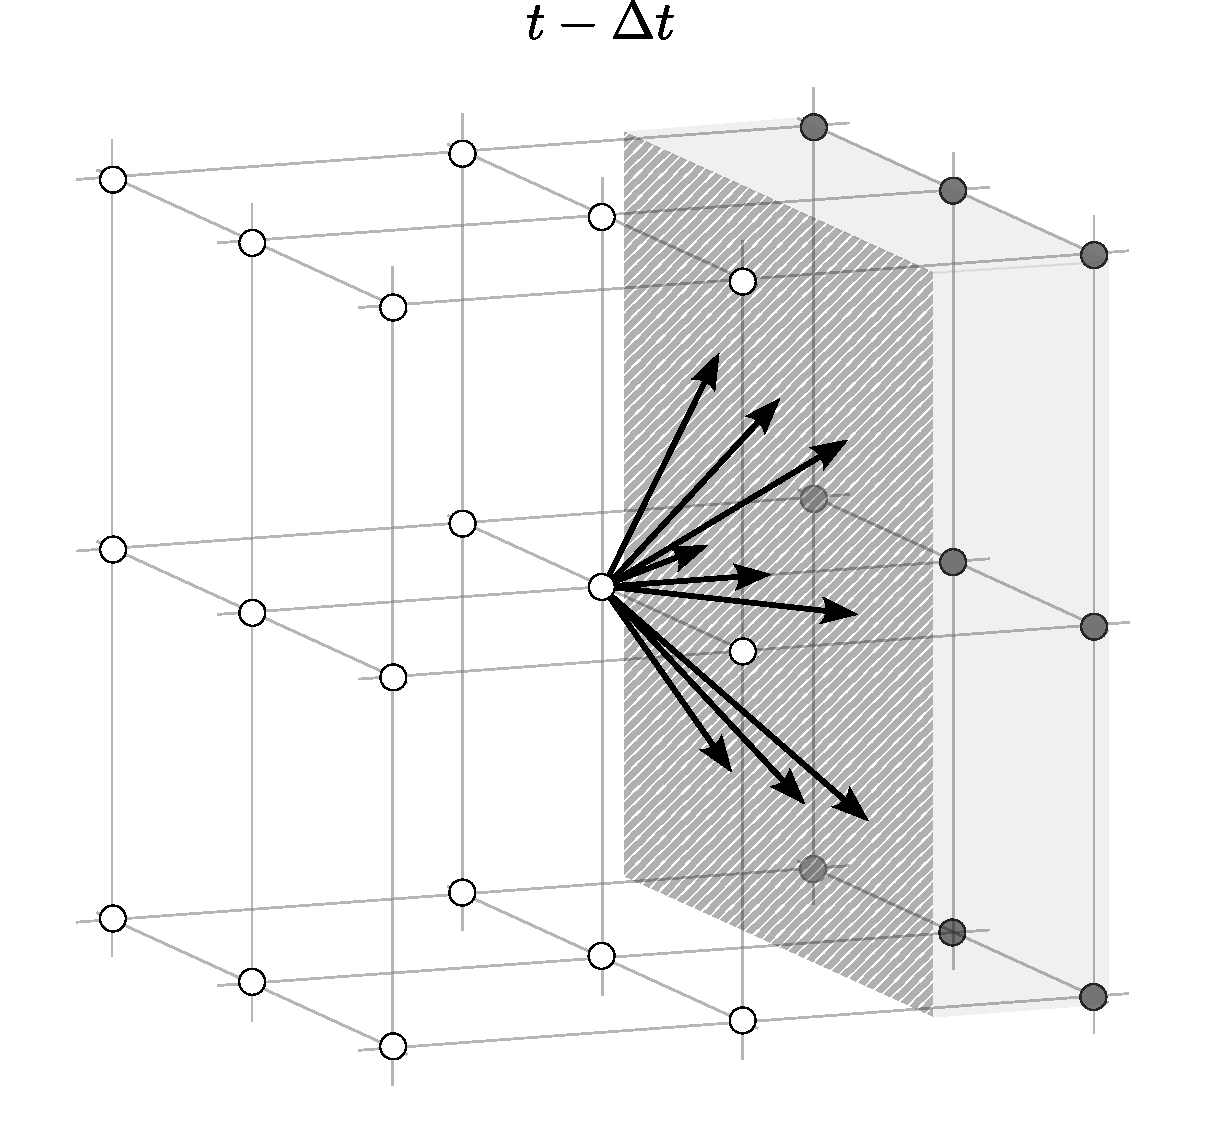
\includegraphics[width=0.9\textwidth, trim={0mm 0mm 0mm 0mm}]{figures/fwbba.pdf}
		\caption{Step before the streaming at time $t - \Delta t$.}
		\label{fig:bba}
	\end{subfigure}
	\begin{subfigure}{0.48\textwidth}
		\centering
		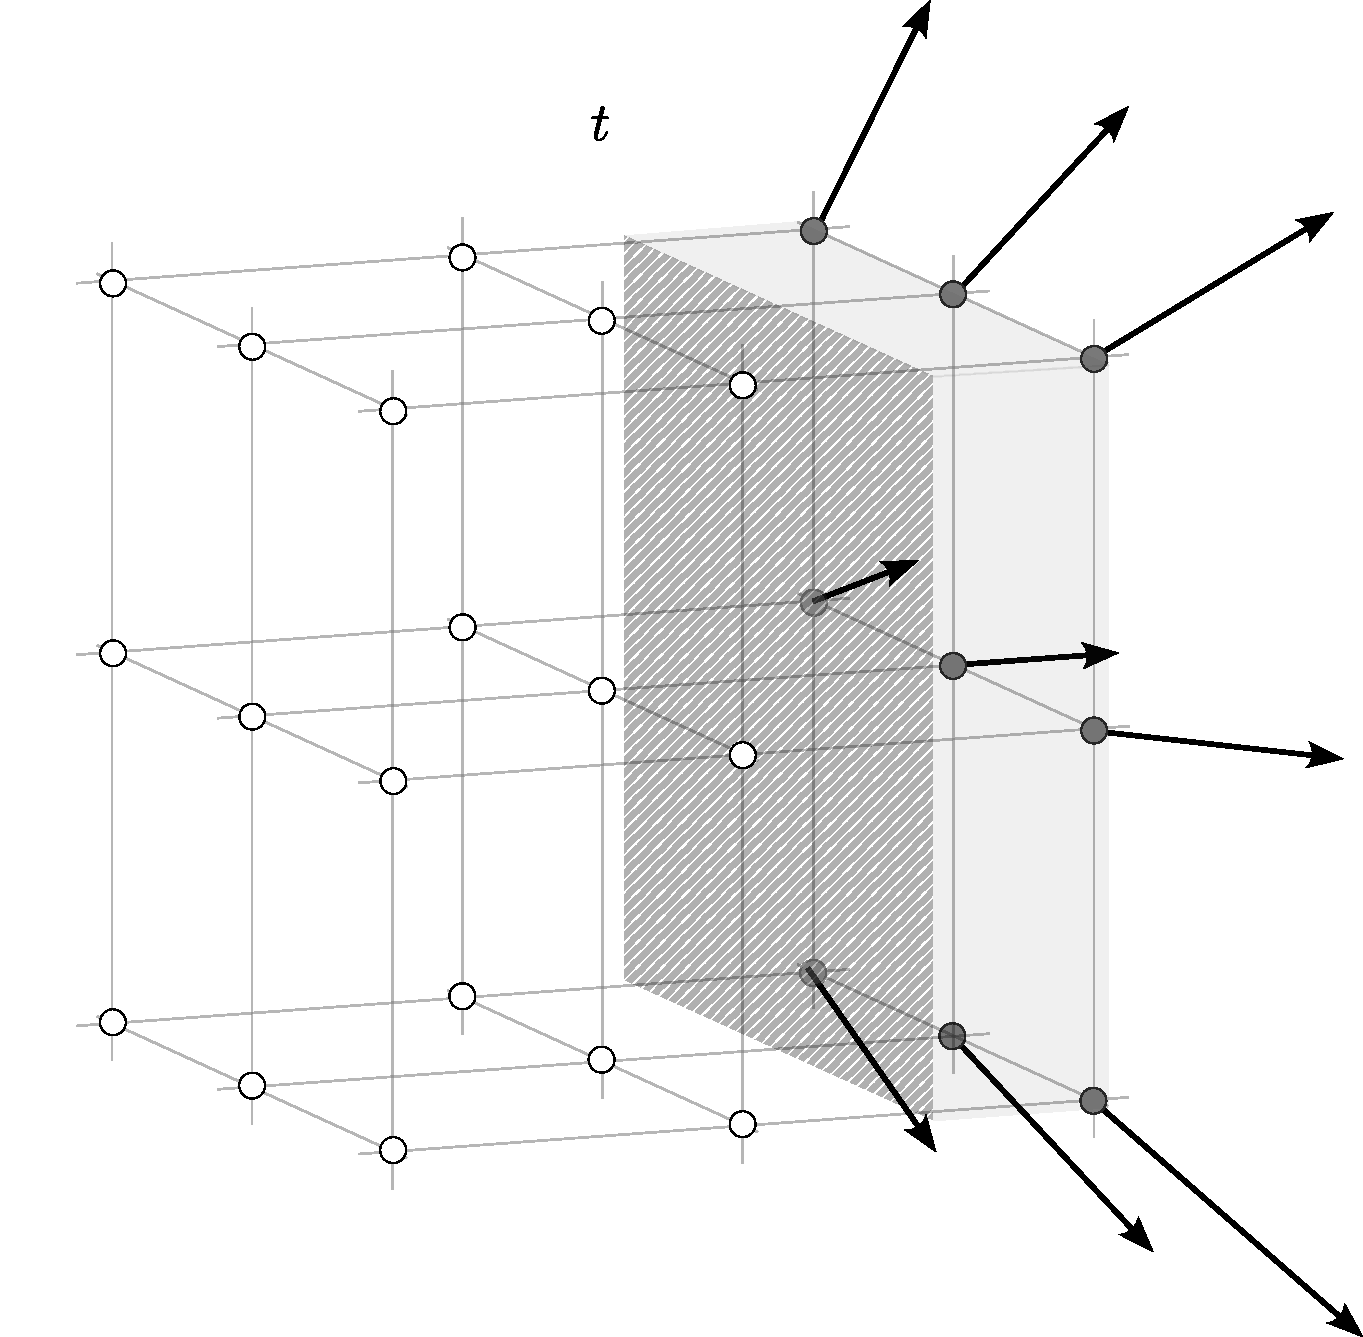
\includegraphics[width=0.9\textwidth, trim={0mm 0mm 0mm 0mm}]{figures/fwbbb.pdf}
		\caption{Step after streaming at time $t$.}
		\label{fig:bbb}
	\end{subfigure}
	\par\bigskip
	\par\bigskip
	\begin{subfigure}{0.48\textwidth}
		\centering
		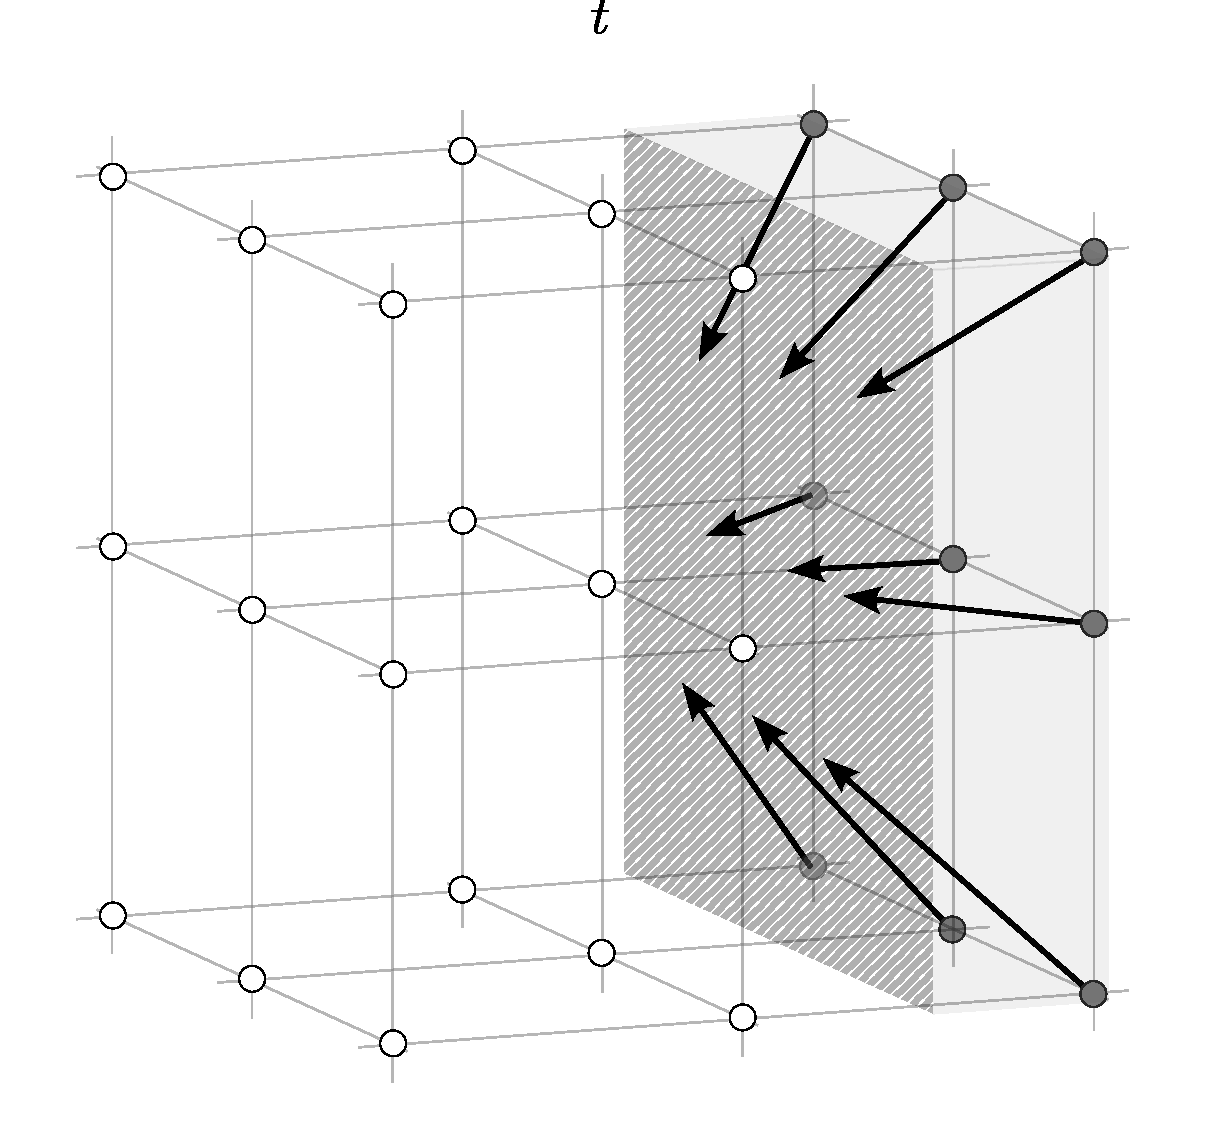
\includegraphics[width=0.9\textwidth, trim={0mm 0mm 0mm 0mm}]{figures/fwbbc.pdf}
		\caption{The distribution functions are reversed.}
		\label{fig:bbc}
	\end{subfigure}
	\begin{subfigure}{0.48\textwidth}
		\centering
		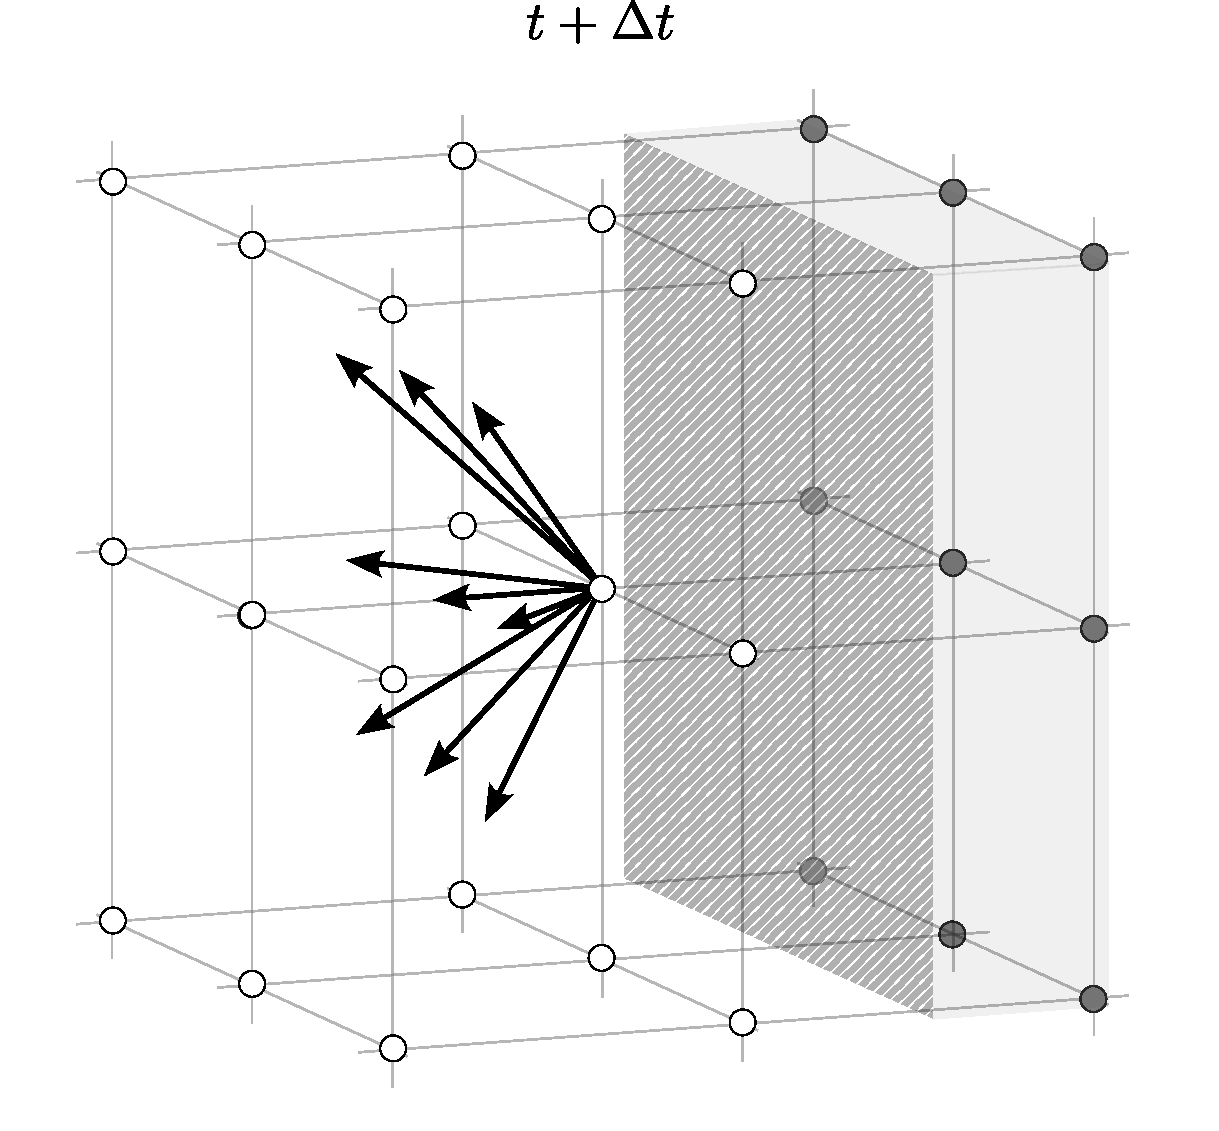
\includegraphics[width=0.9\textwidth, trim={0mm 0mm 0mm 0mm}]{figures/fwbbd.pdf}
		\caption{Step after the streaming at time $t + \Delta t$.}
		\label{fig:bbd}
	\end{subfigure}
	
	\caption{Schematic representation of the fullway bounce-back boundary condition for the D3Q27 velocity model. White points represent the fluid sites and gray points represent the wall sites, with the wall shown as a gray plane.}
	\label{fig:fbb}
\end{figure}


It is worth noting that there is also a \textit{halfway} variant of the bounce-back boundary condition, which requires only one time step for its realization. Details can be found, for example, in \cite{Kruger}. However, in this work, we will limit ourselves to the fullway variant.

\subsubsection{Equilibrium boundary condition}\label{equilibrium bc}
One option for approximating unknown distribution function values at the boundary nodes is to use the equilibrium distribution function, defined as \cite{PE}
\begin{equation}
	f_i(\vec{x}, t)=f_{i}^{\text{(eq)}}(\rho(\vec{x}, t), \vec{u}(\vec{x}, t)), \hspace{2mm}  \forall k \in \{1,\dots,27\}, \forall t \in \hat{\mathcal{I}}.
\end{equation}
The advantage of this approximation is its simple implementation, while the disadvantage is the neglect of the non-equilibrium part of the distribution function \cite{PE}.
